\documentclass[dvipsnames]{standalone}

\usepackage{tikz}
\usepackage{url}
\usetikzlibrary{shapes, shapes.misc}
\usepackage{xcolor}


\definecolor{lightturkis}{HTML}{03bdeb}
\definecolor{turkis}{HTML}{2cb1d2}
\definecolor{darkturkis}{HTML}{4ca2b8}

\definecolor{lightblue}{HTML}{3011e3}
\definecolor{blue}{HTML}{4d37ca}
\definecolor{darkblue}{HTML}{6154b0}

\definecolor{lightpurple}{HTML}{9e03e6}
\definecolor{purple}{HTML}{992bcc}
\definecolor{darkpurple}{HTML}{924ab3}


\definecolor{lightorange}{HTML}{FFA364}
\definecolor{orange}{HTML}{FF6802}
\definecolor{darkorange}{HTML}{9C3F00}


\begin{document}
\newcommand{\subjektbuntraw}[4][white]{
	\begin{tikzpicture}[scale=0.4]
	
	\draw[fill=#2,thick]  (0,0.5) rectangle (6,2.5);
	\draw[fill=#3,thick]  (3,1) rectangle (9,3);
	\draw[fill=#4,thick]  (1,1.5) rectangle (7,3.5);
	\end{tikzpicture}
}

\newcommand{\subjektraw}[1][white]{
	\begin{tikzpicture}[scale=0.3]
	\draw[fill=#1,thick]  (0,0) rectangle (3,4);
	\draw[fill=#1,thick]  (-0.5,0.5) rectangle (2.5,4.5);
	\draw[fill=#1,thick]  (-1,1) rectangle (2,5);
	\end{tikzpicture}
}


\newcommand{\odmlraw}[1][White]{
\begin{tikzpicture}
\begin{scope}[scale=0.4]
\node (State00) [circle, radius=0.8cm, draw=Black, fill=Black!90] {} [-, line width=1, sibling distance=2cm, level distance=2cm] 
    child{node (State01) [rectangle, draw=Black, fill=#1, minimum width=0.3cm, minimum height=0.3cm] {}}
    child{node (State01) [rectangle, draw=Black, fill=#1, minimum width=0.3cm, minimum height=0.3cm] {}};
\end{scope}
\end{tikzpicture}

}

\newcommand{\odmlbuntraw}[3]{
	\begin{tikzpicture}
	\begin{scope}[scale=0.5]
	\draw[darkblue,fill=#2]  (0,0) rectangle (4,5/3);
	\draw[blue,fill=#2]  (0,5/3) rectangle (4,10/3);
	\draw[lightblue,fill=#3]  (0,10/3) rectangle (4,15/3);
	\draw  (0,0) rectangle (4,5);
	\end{scope}
	\end{tikzpicture}
}

\newcommand{\odmltext}[2][below]{
	\usetikzlibrary{positioning}
\begin{tikzpicture}
	\node(r) {\odmlraw};
	\node[align=center, #1= -0.3em of r] (t) {#2};
\end{tikzpicture}
}

\newcommand{\odmlbunttext}[5][below]{
	\usetikzlibrary{positioning}
	\begin{tikzpicture}
	\node(r) {\odmlbuntraw{#3}{#4}{#5}};
	\node[align=center, #1= -0.3em of r] (t) {#2};
	\end{tikzpicture}
}
\newcommand{\subjekttext}[2][below]{
	\usetikzlibrary{positioning}
	\begin{tikzpicture}
	\node(r) {\subjektraw[red]};
	\node[align=center, #1= -0.3em of r] (t) {#2};
	\end{tikzpicture}
}

\newcommand{\subjektbunttext}[6][below]{
	\usetikzlibrary{positioning}
	\begin{tikzpicture}
	\node(r) {\subjektbuntraw{#4}{#5}{#6}};
	\node[align=center, #1= +0.3em of r] (t) {\textit{#3}};
	\node[align=center, above= -0em of t] (u) {\textbf{#2}};
	\end{tikzpicture}
}

\newcommand{\scripts}[2][below]{
	\usetikzlibrary{positioning}
	\begin{tikzpicture}
	\node(r) {\subjektraw};
	\node[align=center, #1= -0.3em of r] (t) {#2};
	\end{tikzpicture}
}

\newcommand{\manual}[2][below]{
	\usetikzlibrary{positioning}
	\begin{tikzpicture}
	\node(r) {
\includegraphics[width=1.5cm]{icons/hand}};
	\node[align=center, #1= -0.3em of r] (t) {#2};
	\end{tikzpicture}
}

\newcommand{\filledtemplates}[2][below]{
	\usetikzlibrary{positioning}
	\begin{tikzpicture}
	\node[draw, thick, fill=White](r) {\odmlraw[turkis]};
	\node[draw, thick, fill=White, yshift=1em, xshift=-1em](s) {\odmlraw[blue]};
	\node[draw, thick, fill=White, yshift=2em, xshift=-2em](t) {\odmlraw[purple]};
	\node[align=center, #1= -0em of r] (t) {#2};
	\end{tikzpicture}
}

\newcommand{\odMLtree}{
	\usetikzlibrary{positioning}
	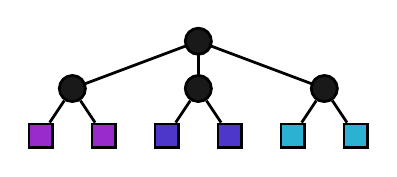
\begin{tikzpicture}
	\begin{scope}[scale=0.4]
	\node (State0) [-,circle, radius=0.8cm, draw=Black, fill=Black!90, growth parent anchor=south] {} [-, line width=1, sibling distance=4cm]
	    child{ [sibling distance=2cm]
		  node (State00) [circle, radius=0.8cm, draw=Black, fill=Black!90] {} 
		  child{node (State000) [rectangle, draw=Black, fill=purple, minimum width=0.3cm, minimum height=0.3cm] {}}
		  child{node (State001) [rectangle, draw=Black, fill=purple, minimum width=0.3cm, minimum height=0.3cm] {}}
	    }
	    child{ [sibling distance=2cm]
		  node (State01) [circle, radius=0.8cm, draw=Black, fill=Black!90] {}
		  child{node (State011) [rectangle, draw=Black, fill=blue, minimum width=0.3cm, minimum height=0.3cm] {}}
		  child{node (State011) [rectangle, draw=Black, fill=blue, minimum width=0.3cm, minimum height=0.3cm] {}}
	    }
	    child{ [sibling distance=2cm]
		  node (State02) [circle, radius=0.8cm, draw=Black, fill=Black!90] {}
		  child{node (State021) [rectangle, draw=Black, fill=turkis, minimum width=0.3cm, minimum height=0.3cm] {}}
		  child{node (State021) [rectangle, draw=Black, fill=turkis, minimum width=0.3cm, minimum height=0.3cm] {}}
	    };
	\end{scope}
	\end{tikzpicture}
}


\begin{tikzpicture}
\usetikzlibrary{positioning}
\begin{scope}[scale=1]
	\node[draw, fill=gray!20, midway] (collection) {
		\odmltext[right]{\textbf{odML template}}
		\scripts[right]{\parbox{7em}{\textbf{scripted\\enrichment}}}
		\manual[right]{\parbox{7em}{\textbf{manual\\enrichment}}}
	};
	
	\node[below= 2cm of collection](enriched) {
		\filledtemplates[right]{\parbox{7em}{\textbf{complete metadata collections}}}
	};

	\draw[->, line width=1] (collection) -- (enriched);
	
	\node[draw, fill=gray!20, below=2cm of enriched] (integration) {
		\begin{tikzpicture}
		\node[draw, circle, thick, fill=Black, minimum width=1cm](r) {};
		\draw (r) node[anchor=center, cross out, draw=white, line width=2mm, minimum size=0.5cm, inner sep=0pt, outer sep=0pt, rotate=45] {};
		\node[align=center, right= -0.0em of r] (t) {\parbox{7em}{\textbf{integration}}};
		\end{tikzpicture}
	};
	
	\draw[->, line width=1] (collection) -- (enriched);
	
	\draw[->, line width=1] (enriched) -- (integration);
	
	\node[above= 2cm of collection](s1) {\subjektbunttext[above]{metadata collection B}{e.g. recording day 2}{darkblue}{blue}{lightblue}};
	\node[left=of s1](s2) {\subjektbunttext[above]{metadata collection A}{e.g. recording day 1}{darkpurple}{purple}{lightpurple}};
	\node[right=of s1](s3) {\subjektbunttext[above]{metadata collection C}{e.g. recording day 3}{darkturkis}{turkis}{lightturkis}};
	
	\draw[->, line width=1] (s1) -- (collection);
	\draw[->, line width=1] (s2) -- (collection);
	\draw[->, line width=1] (s3) -- (collection);
	
	\node[below=2cm of integration] (end) {\odMLtree};
	\node[right= 0em of end] {\parbox{10em}{\textbf{complete odML\\collection}}};
	
	\draw[->, line width=1] (integration) -- (end);
	
% 	\node[below= 2cm of integration](o1) {\odmlbunttext[below]{odML file subject 2}{lightblue}{blue}{darkblue}};
% 	\node[left=of o1](o2) {\odmlbunttext[below]{odML file subject 1}{lightpurple}{purple}{darkpurple}};
% 	\node[right=of o1](o3) {\odmlbunttext[below]{odML file subject 3}{lightturkis}{turkis}{darkturkis}};
% 	
% 	\draw[<-, line width=1] (o1) -- (integration);
% 	\draw[<-, line width=1] (o2) -- (integration);
% 	\draw[<-, line width=1] (o3) -- (integration);
	
\end{scope}
\end{tikzpicture}

\end{document}	

